\section{Εισαγωγή}

Τα συστήματα αυτοματισμού είναι πλέον μέρος της καθημερινότητας μας. Συναντάμε συνέχεια, χωρίς
απαραίτητα να το συνειδητοποιούμε κάποιου είδος σύστημα το οποίο είναι προγραμματισμένο να εκτελεί
μια διεργασία με βάση ορισμένες συνθήκες του εξωτερικού του περιβάλλοντος. Το παραπάνω έχει μεγάλο
αντίκτυπο στον κόσμο το οποίο γίνεται ξεκάθαρο με την ραγδαία εξέλιξη του IoT (Internet of Things).
Περιτριγυριζόμαστε από συσκευές οι οποίες λειτουργούν ως συστήματα αυτοματισμού αλλά παράλληλα
επικοινωνούν με το Cloud. Από την πλευρά των προγραμματιστών προσφέρονται άπειρες συσκευές με τις
δικές τους ιδιαιτερότητες και άπειρα εργαλεία που λειτουργούν στην κάθε συσκευή.
Δεν είναι όμως ξεκάθαρο το πιο είναι καλύτερο για κάθε use-case. Στην εκάστοτε
εργασία θα χρησιμοποιήσουμε τον μικροελεγκτή ESP32C6-DevKitC-1 και θα γίνει μια απόπειρα
σύγκρισης τριών διαφορετικών οικοσυστημάτων προγραμματισμού (Arduino, Rust-Embassy, ESP-IDF).
Με σκοπό την πλήρης διαφάνεια των αποτελεσμάτων το παρακάτω κεφάλαιο εξηγεί την απαραίτητη
θεωρία για την κατανόηση των συστημάτων αυτοματισμού, του μικροελεγκτή και τα KPI (Key
Perfomance Indicators) που θα μετρήσουμε.

\subsection{Συστήματα Αυτοματισμού}

\begin{figure}[h!]
\centering
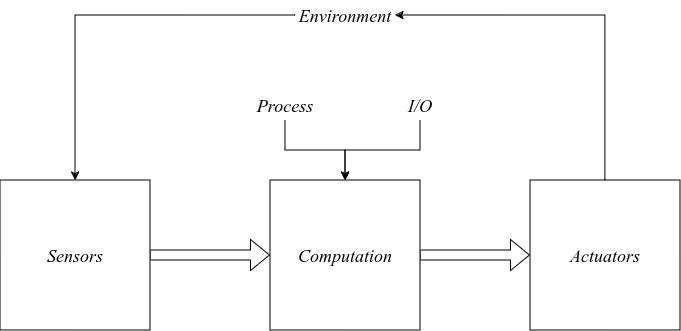
\includegraphics[scale=0.4]{images/introduction/as_elements.png}
\caption{Αναπαράσταση βασικών στοιχείων συστημάτων αυτοματισμού.}
 \label{fig:as_elements}
\end{figure}

Ένα σύστημα αυτοματισμού είναι ένα σύστημα που αποτελείτε από τρία
βασικά στοιχεία:

\begin{enumerate}
\item Τους σένσορες ή αισθητήρες, που λαμβάνουν δεδομένα από το
εξωτερικό τους περιβάλλων και παράγουν ένα όσο το δυνατόν πιο
αξιόπιστο αναλογικό ή ψηφιακό σήμα.
\item Ένα υπολογιστικό σύστημα, για παράδειγμα έναν μικροελεγκτή το
οποίο μπορεί να χρησιμοποιήσει το σήμα των αισθητήρων για
υπολογισμούς, επεξεργασία ή I/O.
\item Το στοιχείο δράσης ή ενεργοποιητής, που με βάση των υπολογισμών
του υπολογιστικού συστήματος ενεργοποιούνται ή παραμένουν
αδρανής. Αυτό το στοιχείο αποτελεί την έξοδο του συστήματος
αυτοματισμού και είναι αυτό το οποίο έχει συνήθως αντίκτυπο στο
εξωτερικό του περιβάλλων.
\end{enumerate}

Το υπολογιστικό σύστημα μπορεί να χρησιμοποιηθεί για να παίρνει
αποφάσεις με βάση των τιμών που δέχεται από τους αισθητήρες και εκεί
φαίνεται η πραγματική χρησιμότητα των αυτόματων συστημάτων. Πολλές
φορές με βάση την λήψη αποφάσεων (υπολογισμών) το αποτέλεσμα του
στοιχείου δράσης χρειάζεται να επιστρέψει στην είσοδο του συστήματος,
για παράδειγμα εάν χρειάζεται να ρυθμιστεί ένας σένσορας δυναμικά. Σε
αυτήν την περίπτωση το σύστημα λέγεται σύστημα ανατροφοδότησης ή
αλλιώς σύστημα κλειστού βρόχου \figref{fig:as_feedback}.

\begin{figure}[h!]
\centering
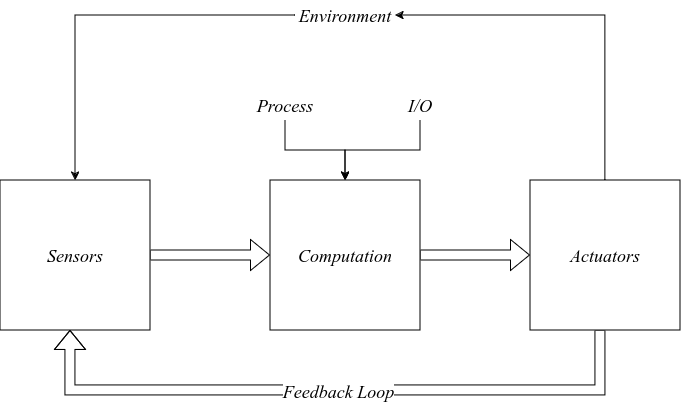
\includegraphics[scale=0.4]{images/introduction/as_feedback.png}
\caption{Σύστημα κλειστού βρόχου.}
 \label{fig:as_feedback}
\end{figure}

Για την παρούσα εργασία μας ενδιαφέρει κυρίως το υπολογιστικό
σύστημα. Συγκεκριμένα, μας ενδιαφέρει ο προγραμματισμός του
μικροελεγκτή ESP32C6, προκύπτει όμως ένα πρόβλημα. Τα συστήματα
αυτοματισμού δεν περιλαμβάνουν την θεωρία προγραμματισμού
μικροελεγκτών, αυτό ισχύει διότι είναι ένα abstraction (αφαίρεση) που
αφαιρεί την ανάγκη συγκεκριμένου υπολογιστικού συστήματος.  Για
παράδειγμα θα μπορούσαμε να χρησιμοποιήσουμε ένα Raspberry Pi, αυτό
δεν θα άλλαζε το γεγονός ότι λειτουργούμε σε ένα σύστημα αυτοματισμού
ασχέτως από το ότι χρησιμοποιούμε ένα single-board computer (SBC) αντί
για ένα micro-controller unit (MCU). Εδώ προκύπτει το ερώτημα, πια η
διαφορά;

\subsection{Embedded Systems}

Ο πιο σύγχρονος τρόπος προγραμματισμού παίρνει μέρος συνήθως σε αυτό
που αποκαλούμε user-space ενός λειτουργικού συστήματος.  Στο
user-space το OS (Operating System) αναλαμβάνει ένα πολύ μεγάλο μέρος
της πολυπλοκότητας του προγραμματισμού. Η δημιουργία εικονικής μνήμης,
η δυνατότητα παράλληλου προγραμματισμού, η διαχείριση μνήμη σορού
(heap memory) είναι όλα προβλήματα που αντιμετωπίζονται σχεδόν
αυτόματα πλέον. Επίσης μέσο του λειτουργικού συστήματος αποκρύβονται
οι λεπτομέρειες του hardware, τα πάντα σχεδόν προσφέρονται ως ψηφιακά
API (Application Programming Interface), τα οποία χτίζονται το ένα
πάνω στο άλλο.  Με κάθε πρόσθεση επιπέδου αφαίρεσης χάνετε λίγο
παραπάνω η ικανότητα πλήρης διαχείρισης του hardware με το θετικό ότι
σε γενικές γραμμές κάνει την ζωή του προγραμματιστή πιο εύκολη. Είναι
ξεκάθαρο λοιπόν ότι τα abstraction layers είναι χρήσιμα, αλλά είναι
δίκοπο μαχαίρι. Από την μια πλευρά η υλοποίηση των περισσότερων
εφαρμογών γίνεται απίστευτα πιο εύκολη. Από την άλλη, τι γίνεται όταν
πραγματικά χρειαζόμαστε να επικοινωνήσουμε με το hardware που έχουμε
μπροστά μας;
Πολλές φορές υπάρχουν συστήματα που δεν μπορούν ή δεν χρειάζεται
να τρέξουν ένα ολόκληρο operating system. Πολλές φορές δεν έχουμε την
επιλογή να τρέξουμε κώδικα πάνω σε ένα abstraction. Για παράδειγμα,
συστήματα που βρίσκονται σε απλές συσκευές όπως θερμοστάτες και
ρολόγια όχι μόνο δεν είναι απαραίτητο να τρέχουν OS αλλά πολλές φορές
δεν είναι βέλτιστο. 
Αναφερόμαστε στα συστήματα που δεν χρησιμοποιούν παραδοσιακά OS  ως
embedded systems διότι τα βρίσκουμε συχνά ενσωματωμένα σε μεγαλύτερες συσκευές.

Συνήθως προγραμματίζουμε ένα embedded system στο κύριο μηχάνημα μας
(host machine) το οποίο είναι λογικά διαφορετικής αρχιτεκτονικής. Αυτό
σημαίνει ότι πρέπει να μετατρέψουμε τον πηγαίο κώδικα της high level
γλώσσας που χρησιμοποιούμε στην αντίστοιχη γλώσσα που καταλαβαίνει ο
εξωτερικός επεξεργαστής. Αυτή η διαδικασία λέγεται
cross-compiling. Μάλιστα είναι απαραίτητο να δώσουμε στο πρόγραμμα τις
απαραίτητες τοποθεσίες στην μνήμη στην οποία θα εκτελεί εντολές ή θα
αποθηκεύει στατικά δεδομένα, αυτή είναι δουλειά του
linker. Αναλυτικότερα ο πηγαίος κώδικας, μαζί
με ότι βιβλιοθήκες χρησιμοποιούνται περνάνε από τον compiler και
πρώτα προεπεξεργάζονται και ενώνονται σε μια δομή.
Μεταφράζονται αργότερα στην assembly που καταλαβαίνει το target
μηχάνημα και ο assembler τα μετασχηματίζει σε ένα ή περισσότερα
Relocatable Object αρχεία, δηλαδή συλλογές από bytes που
αντιπροσωπεύουν τον κώδικα στην target γλώσσα. Έπειτα τα object files
περνάνε από τον linker ο οποίος ανάλογα με τις ρυθμίσεις του οργανώνει
το αρχείο και προσθέτει απαραίτητα δεδομένα για να δημιουργήσει ένα
εκτελέσιμο για το target μηχάνημα πρόγραμμα, για παράδειγμα ένα ELF32 \figref{fig:compilation_stages}.

\begin{figure}[h!]
\centering
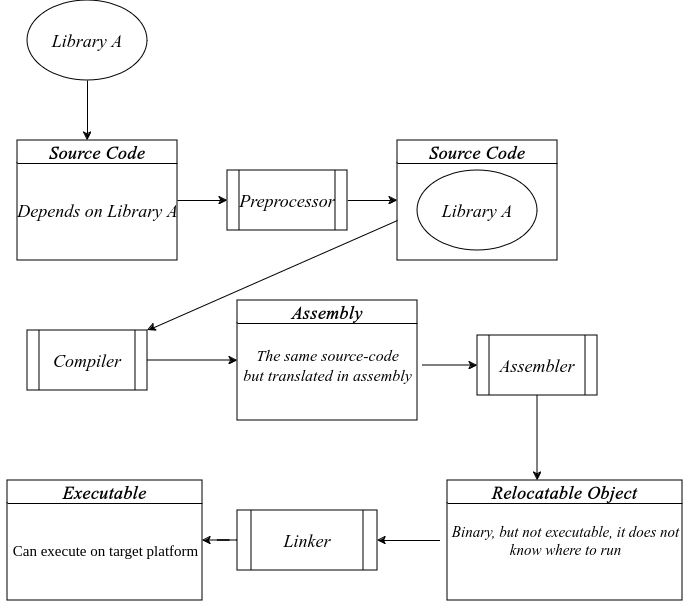
\includegraphics[scale=0.4]{images/introduction/compilation_stages.png}
\caption{Στάδια μεταγλώττισης.}
 \label{fig:compilation_stages}
\end{figure}

\newpage

Η πραγματικότητα είναι ότι πλέον, ειδικά για μικρά projects, η διαδικασία
των σταδίων μεταγλώττισης είναι αυτοματοποιημένη και γίνονται όλα μέσο του
οικοσυστήματος όπως θα δούμε αργότερα. Όμως εξακολουθεί να είναι ιδιαίτερα χρήσιμη η γνώση
τους και απασχολεί πολύ τον κόσμο της πληροφορικής ακόμα και σήμερα, για λόγους βελτιστοποίησης 
και debugging.

Εφόσον έχουμε δημιουργήσει ένα εκτελέσιμο αρχείο πρέπει με κάποιο τρόπο να το στείλουμε στην συσκευή.
Συνήθως χρησιμοποιούμε κάποιο σειριακό πρωτόκολλο, τύπου USB το οποίο εσωτερικά συνδέεται με κάποιου είδους
μη πτητικής μνήμης για να το αποθηκεύσει \figref{fig:embedded_workflow}. Αυτό έχει ως αποτέλεσμα το πρόγραμμα να διατηρείτε ανεξαρτήτως
αν αργότερα κάνουμε επανεκκίνηση ή τερματίσουμε την συσκευή.

\begin{figure}[h!]
\centering
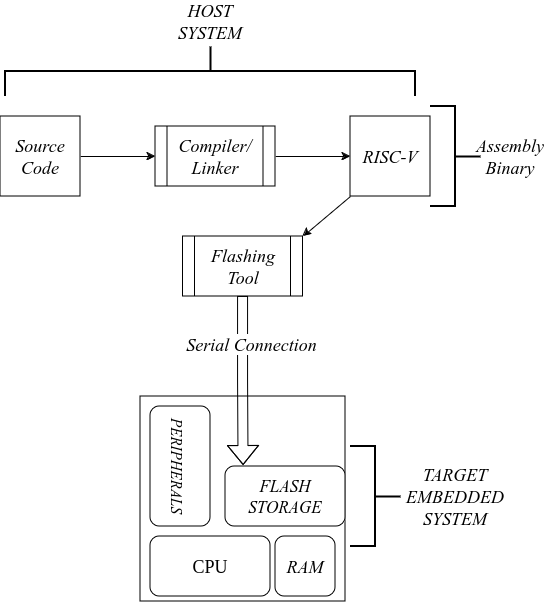
\includegraphics[scale=0.4,angle = 90]{images/introduction/programming_embedded.png}
\caption{Development workflow}
 \label{fig:embedded_workflow}
\end{figure}

\newpage

Όταν ενεργοποιήσουμε την μηχανή τα απαραίτητα στοιχεία από την μη πτητική μνήμη
αντιγράφονται στην προσωρινή και ο καταχωρητής program counter του επεξεργαστή
δείχνει στην διεύθυνση μνήμης στην οποία βρίσκεται η πρώτη εντολή του πρώτου
προγράμματος που θα τρέξει. Συνήθως αυτό είναι κάποιου είδους bootloader, αλλά
στα ενσωματωμένα συστήματα δεν είναι πάντα αυτή η περίπτωση και τρέχει το firmware
που έχουμε γράψει κατευθείαν. 

\begin{figure}[h!]
\centering
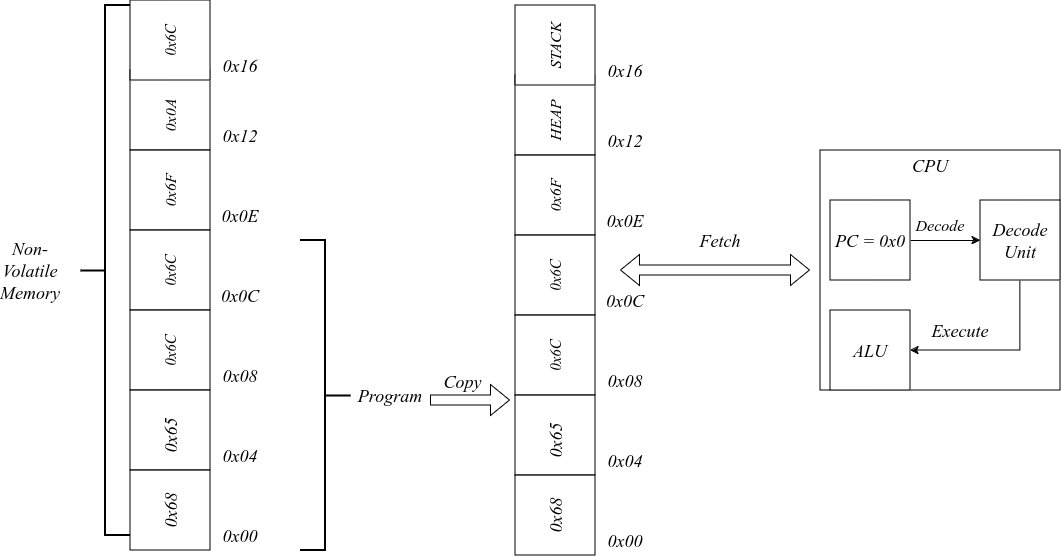
\includegraphics[scale=0.4,angle=90]{images/introduction/instruction_cycle.drawio.png}
\caption{Κύκλος εντολών μηχανής}
 \label{fig:instruction_cycle_workflow}
\end{figure}

Αξίζει να σημειωθεί ότι δεν είναι πάντα ξεκάθαρο το πως η μη πτητική μνήμη αντιγράφετε στην
προσωρινή εξαρχώς, μπορεί οι μνήμες να έχουν ενσωματωμένο firmware και
να επικοινωνούν με σύνδεση τύπου I2C ή UART ή πιο λογικό να είναι ο
bootloader του επεξεργαστή σε μια ανεξάρτητη ROM (Read Only Memory)
σταθερής διεύθυνσης και μεγέθους και να είναι αυτός υπεύθυνος για την
επικοινωνία. Παράλληλα, υπάρχουν πολλοί καταχωρητές οι οποίοι διαχειρίζονται
την κατάσταση (state) του επεξεργαστή και κατά συνέπεια ολόκληρου του συστήματος. Ο program counter
αναφέρετε διότι διατηρείτε σε πρακτικά όλες τις αρχιτεκτονικές. 

Είναι σημαντικό να γνωρίζουμε επίσης ότι μια εντολή δεν εκτελείτε
κατευθείαν. Όπως αναπαριστά το παραπάνω διάγραμμα, πρώτα ο
επεξεργαστής διαβάζει την εντολή από την μνήμη (fetch). Έπειτα την
αποσπά για να την κατανοήσει (decode). Θυμόμαστε ότι έχουμε
αποθηκεύσει το εκτελέσιμο αρχείο, δηλαδή αυτό που είναι κατανοητό στην
μηχανή, σε δυαδική μορφή, όχι σε γραμματοσειρά που είναι κατανοητή
στους ανθρώπους. Για παράδειγμα οι εντολές της αρχιτεκτονικής RISC-V
32bit έχουν σταθερό μέγεθος και αναπαριστούν μια αριθμητική τιμή $x \in
[0, 2^{31}] \subseteq \mathbb{N}_0$. Ο αριθμός αυτός στην δυαδική του μορφή, μπορεί να
διαχωριστεί σε $n\in\mathbb{N}$ θραύσματα, συνήθως τα λέμε nibbles, μέσο bit operations και εξηγούν στον
επεξεργαστή τι πρέπει να κάνει. Στην πολύ συχνή εντολή
\verb|add t0, t1, t2|, στην οποία προσθέτουμε την τιμή του καταχωρητή
$t1$ με την τιμή του καταχωρητή $t2$ και την αποθηκεύουμε στον t0, ένα
unit του επεξεργαστή κάνει τις παρακάτω πράξεις για να την
αποκωδικοποιήσει.

\vspace{0.5cm}

\begin{math}
  Bits_{0-31} \text{ is stored in memory and then enters a unit capable of decoding RISC-V instructions:}  \newline
  Bits_{0-31} = \verb|add t0, t1, t2| = 0x007302b3_{(16)} \newline
  Bits_{0-6} = Bits_{0-31} \BitAnd 0x7F_{(16)} \rightarrow \text{opcode} \newline
  Bits_{7-11} = (Bits_{0-31} \ShiftRight 7_{(10)}) \BitAnd 0x1F_{(16)} \rightarrow \text{destination register} \newline
  Bits_{12-14} = (Bits_{0-31} \ShiftRight 12_{(10)}) \BitAnd 0x7_{(16)} \rightarrow \text{operation (addition)} \newline
  Bits_{15-19} = (Bits_{0-31} \ShiftRight 15_{(10)}) \BitAnd 0x1F_{(16)} \rightarrow \text{source register 1} \newline
  Bits_{20-24} = (Bits_{0-31} \ShiftRight 20_{(10)}) \BitAnd 0x1F_{(16)} \rightarrow \text{source register 2} \newline
  Bits_{25-31} = (Bits_{0-31} \ShiftRight 25_{(10)}) \BitAnd 0x7F_{(16)} \rightarrow \text{addition variant} \newline
\end{math}

Η λογική αποκωδικοποίησης είναι ίδια σε πρακτικά όλες τις
αρχιτεκτονικές όμως το μέγεθος μιας εντολής δεν είναι σε όλες
σταθερό. Τέλος, παίρνουν μέρος οι αριθμητικές πράξεις ή το I/O με βάση
τα αποτελέσματα του decoding (execute).

Η καθυστέρηση που έρχεται ως επίπτωση των παραπάνω πράξεων μπορεί να
φαίνεται στην αρχή σαν μεγάλη υπερφόρτωση του υπολογιστικού συστήματος
και πράγματι για παλαιότερες αρχιτεκτονικές ήταν. Το λεγόμενο
Instruction Cycle όμως (Fetch \rightarrow Decode \rightarrow Execute)
που μόλις αναλύσαμε έχει οριστεί για έναν πολύ συγκεκριμένο
λόγο. Ουσιαστικά ο επεξεργαστής εκμεταλλεύεται την καθυστέρηση που
παίρνει μέρος υλοποιώντας μια δομή, για τους σκοπούς μας ένα
pipeline. Κάθε φορά που αλλάζει το state μιας εντολής προχωράει
στο pipeline και προσθέτετε μια καινούργια εντολή στην αρχικοποιημένη της
κατάσταση. Αυτό δίνει την ψευδαίσθηση παραλληλισμού στο επίπεδο του επεξεργαστή
και είναι ένας από τους πολλούς λόγους που σύγχρονα προγράμματα μπορούν να τρέχουν
τόσο γρήγορα χωρίς απαραίτητα να τρέχουν πάνω σε ένα runtime.

Η περίπτωση του ESP32C6 είναι ότι αν και είναι πανίσχυρος για μικροελεγκτής ανάλογα
με το framework περιέχει μινιμαλιστικά, στην καλύτερη περίπτωση, abstractions.

\begin{figure}[!htb]
    \centering
    \begin{minipage}{0.49\textwidth}
        \centering
        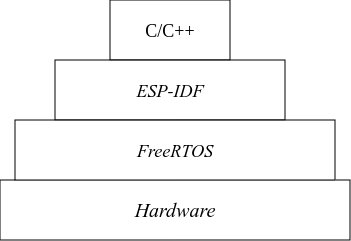
\includegraphics[scale=0.4]{images/introduction/idf_layers}
        \caption{ESP-IDF Abstraction Layers}
        \label{fig:idf_layers}
      \end{minipage}  
    \begin{minipage}{0.49\textwidth}
        \centering
        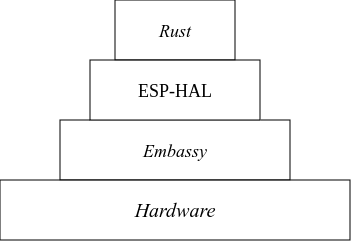
\includegraphics[scale=0.4]{images/introduction/rust_layers}
        \caption{Embassy Abstraction Layers}
        \label{fig:rust_layers}
      \end{minipage}  
    \begin{minipage}{0.49\textwidth}
      \centering
        \vspace{0.5cm}
        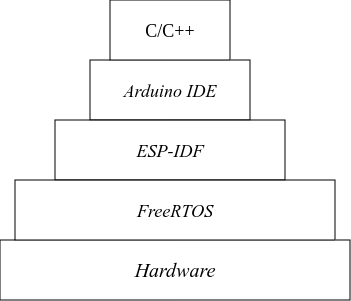
\includegraphics[scale=0.4]{images/introduction/arduino_layers}
        \caption{Arduino Abstraction Layers}
        \label{fig:arduino_layers}
    \end{minipage}%
\end{figure}



